\section{8 de febrero de 2021}

\subsection{Compactos}
\begin{definition}
Sea $A$ un subconjunto del espacio métrico M. Decimos que la familia de abiertos $\{G_1\}_{i\in I}$ de $M$ es una cubierta de $A$, si
$$A\subset \bigcup_{i\in I}G_i $$
\end{definition}
\begin{remark}
En el caso de $M$, la cubierta abierta debe cumplir: $M=\bigcup_{i\in I}G_i$
\end{remark}

\begin{definition}
Un subconjunto $A$ del espacio métrico $M$ es \textbf{compacto} si cada abierta de $A$ tiene subcubierta finita \marginnote{Sigue cubriendo al conjunto $A$}. 
\end{definition}

\begin{example}
Sea $k=\{x_1,...,x_n\}$ un subconjunto finito de $\mathbb{R}^n$ y sea $G=\{G_i\}_{i\in I}$ una cubierta abierta de $k$ (i.e. $\bigcup_{i\in I}G_i\supset k$. Dado que $k$ es finito, basta un número finito de los $G_i$ para cubrir a $k\implies k$ es compacto. 
\end{example}
\marginnote{Cerrado y acotado en $\mathbb{R}$ es compacto. En otro caso es necesario investigar}
\begin{example}
Sea $H=[0,\infty)\subseteq \mathbb{R}$ no es compacto. En efecto, sea $G_n =(-1,n), n\in\mathbb{Z}^+$.\newline\newline 
$\implies G=\{G_n\}$ es una cubierta abierta de $H$. Suponga que $\{G_{n_1},G_{n_2},...,G_{n_k}\}$ es una subcolección de $G$. Sea $M=max\{n_1,n_2,...,n_k\}$. Entonces, $G_{n_i}\subseteq G_M, i=1,...,k\implies G_M=\bigcup_{i=1}^k G_{n_i}$, pero en particular, $M\not\in \bigcup_{i=1}^k G_{n_i}\implies \{G_{n_1},...,G_{n_k}\}$ no cubre a $H$. Entonces, $G$ no tiene cubierta finita para $H$. Implica, $H$ no es compacto. 
\end{example}

\begin{example}
Sea $H=(0,1)\subseteq \mathbb{R}$ y considere:
$$G_n(\frac{1}{n},1-\frac{1}{n}), \quad n>2$$

$\implies G=\{G_n\}$ es una cubierta abierta de $H$, pero $G$ no tiene subcubierta finita para $H\implies H$ no es compacta. 
\end{example}

\begin{proposition}
Sea $F$ un subconjunto cerrado de un espacio métrica compacto $M$. Entonces, $F$ es compacto. 
\begin{center}
    

\tikzset{every picture/.style={line width=0.75pt}} %set default line width to 0.75pt        

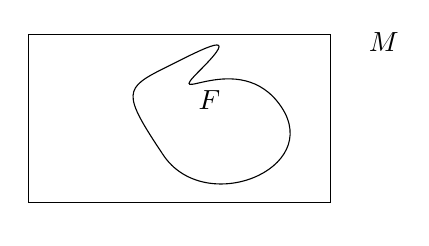
\begin{tikzpicture}[x=0.75pt,y=0.75pt,yscale=-1,xscale=1]
%uncomment if require: \path (0,300); %set diagram left start at 0, and has height of 300

%Shape: Rectangle [id:dp7494793647468762] 
\draw   (24.2,66.2) -- (170,66.2) -- (170,147) -- (24.2,147) -- cycle ;
%Shape: Polygon Curved [id:ds921677921975807] 
\draw   (90.2,82.2) .. controls (110.2,72.2) and (127.2,63.2) .. (107.2,83.2) .. controls (87.2,103.2) and (126.2,71.2) .. (146.2,101.2) .. controls (166.2,131.2) and (109.2,154.2) .. (89.2,124.2) .. controls (69.2,94.2) and (70.2,92.2) .. (90.2,82.2) -- cycle ;

% Text Node
\draw (187,64.1) node [anchor=north west][inner sep=0.75pt]    {$M$};
% Text Node
\draw (105,92.1) node [anchor=north west][inner sep=0.75pt]    {$F$};


\end{tikzpicture}
\end{center}
\end{proposition}

\begin{proof}
Sea $G=\{G_i\}$ una cubierta abierta de F. Como $F^c$ es abierto $\implies (\bigcup_{i\in I}G_i)\cup F^c$ es cubierta abierta de $M$ (i.e $(\bigcup_{i=I}G_i)\cup F^c=M$). Entonces, como $M$ es compacto, existe una subcubierta finita de $M, \{G_{i_1},G_{i_2},..., G_{i_n}, F^c\}$, tal que: 
$$G_{i_1}\cup G_{i_2}\cup... \cup G_{i_n}\cup F^c=M$$
$\implies \{ G_{i_1},...,G_{i_n}$ es una subcubierta finita para $F\implies$ F es compacto. 
\end{proof}

\begin{theorem}[Heine-Borel]
Un subconjunto $S$ de $\mathbb{R}^n$ es compacto ssi es cerrado y acotado. 
\end{theorem}

\begin{example}
\begin{itemize}
    \item (0,1) no es compacto, ya que no es cerrado. 
    \item [0,1] es compacto, por Heine-Borel. 
\end{itemize}
\end{example}

\begin{remark}
\begin{enumerate}
    \item Si $S\subseteq \mathbb{R}$, compacto, $\implies S$ es cerrado y acotado. 
    \item Si $S\mathbb{R}$ es cerrado y acotado $\implies S$ es secuencialmente compacto $\implies  S$ es compacto $\implies S$ es compacto. 
\end{enumerate}
\end{remark}
\marginnote{Teorema de Tíkonov (Tychonoff)- Producto de una colección cualquiera de conjuntos compactos es compacto.}

\begin{remark}
Un espacio métrico $M$ es de Lindelöf si cada cubierta abierta de $M$ tiene una subcubierta contable. 
Un subconjunto $A\subseteq M$ es un  
\end{remark}

\begin{theorem}
Si $S\subseteq\mathbb{R}$ es compacto, entonces $S$ es cerrado y acotado. 
\end{theorem}
\begin{proof}
A probar: $S$ es acotado,\newline 
Considere, para $m\in \mathbb{Z}^+$, $H_m=(-m,m)$. Como cada $H_m$ es abierto  y $ S\subset\bigcup_{i=1}^{\infty} H_m=\mathbb{R} \implies \{H_m:m\in\mathbb{Z}^+\}$ es cubierta abierta de $S$. Como $S$ es compacto $\implies$ Hay una subcubierta finita $\{H_{m_1},...,H_{m_n}\}$ para $S$, i.e $S\subseteq \bigcup_{i=1}^n H_{m_n})=H_m=(-M,M)\implies M$ es acotado.\newline\newline 

A probar: $S$ es cerrado. $\leftrightarrow S^c$ es abierto. 

\begin{center}
    

\tikzset{every picture/.style={line width=0.75pt}} %set default line width to 0.75pt        

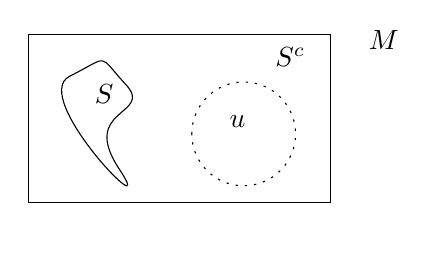
\begin{tikzpicture}[x=0.75pt,y=0.75pt,yscale=-1,xscale=1]
%uncomment if require: \path (0,300); %set diagram left start at 0, and has height of 300

%Shape: Rectangle [id:dp7494793647468762] 
\draw   (24.2,66.2) -- (170,66.2) -- (170,147) -- (24.2,147) -- cycle ;
%Shape: Polygon Curved [id:ds921677921975807] 
\draw   (44.2,86.2) .. controls (64.2,76.2) and (57.2,75.2) .. (71.2,90.2) .. controls (85.2,105.2) and (48.2,101.2) .. (68.2,131.2) .. controls (88.2,161.2) and (24.2,96.2) .. (44.2,86.2) -- cycle ;
%Shape: Circle [id:dp7359910387512897] 
\draw  [dash pattern={on 0.84pt off 2.51pt}] (103,114) .. controls (103,100.19) and (114.19,89) .. (128,89) .. controls (141.81,89) and (153,100.19) .. (153,114) .. controls (153,127.81) and (141.81,139) .. (128,139) .. controls (114.19,139) and (103,127.81) .. (103,114) -- cycle ;

% Text Node
\draw (187,63.1) node [anchor=north west][inner sep=0.75pt]    {$M$};
% Text Node
\draw (55,89.1) node [anchor=north west][inner sep=0.75pt]    {$S$};
% Text Node
\draw (142,71.1) node [anchor=north west][inner sep=0.75pt]    {$S^{c}$};
% Text Node
\draw (120,104.1) node [anchor=north west][inner sep=0.75pt]    {$u$};


\end{tikzpicture}
\end{center}
Sea $u\in S^c$ y considere: 
$$G_n=\{y\in \mathbb{R}:|y-u|> 1/n\}, n\in\mathbb{Z}^+$$
\begin{center}
    

\tikzset{every picture/.style={line width=0.75pt}} %set default line width to 0.75pt        

\begin{tikzpicture}[x=0.75pt,y=0.75pt,yscale=-1,xscale=1]
%uncomment if require: \path (0,300); %set diagram left start at 0, and has height of 300

%Shape: Rectangle [id:dp7494793647468762] 
\draw   (24.2,67.11) -- (223.49,67.11) -- (223.49,218.2) -- (24.2,218.2) -- cycle ;
%Shape: Rectangle [id:dp01772513124623576] 
\draw   (65.21,97.03) -- (190.96,97.03) -- (190.96,190.53) -- (65.21,190.53) -- cycle ;
%Shape: Circle [id:dp6111024653194649] 
\draw  [dash pattern={on 0.84pt off 2.51pt}] (100,145.6) .. controls (100,125.94) and (115.94,110) .. (135.6,110) .. controls (155.26,110) and (171.2,125.94) .. (171.2,145.6) .. controls (171.2,165.26) and (155.26,181.2) .. (135.6,181.2) .. controls (115.94,181.2) and (100,165.26) .. (100,145.6) -- cycle ;

% Text Node
\draw (234.26,73.8) node [anchor=north west][inner sep=0.75pt]    {$\mathbb{R}$};
% Text Node
\draw (197,84.1) node [anchor=north west][inner sep=0.75pt]    {$S^{c}$};
% Text Node
\draw (128,138.1) node [anchor=north west][inner sep=0.75pt]    {$u$};


\end{tikzpicture}
\end{center}
Note que los $G_n$ son abiertos y $\bigcup_{n=1}^\infty G_n=\mathbb{R}-\{u\}$. Como $u\not\in S\implies S\subseteq \bigcup_{n=1}^\infty G_n$. $\implies \{G_n\}$ es una cubierta abierta d $S$. Como $S$ es compacto $\implies \exists m\in\mathbb{Z}^+\ni S\subseteq\bigcup_{n=1}^m G_n=G_m\implies S\cap (u-1/m,u+1/m)=\emptyset\implies (u-1/m,u+1/m)\subset S^c\implies$ es abierto $\implies S$ es cerrado. 
\end{proof}

\begin{remark}
¿Por qué Heine-Borel no aplica en un espacio métrico cualquiera? ¿Se cumple alguna de las implicaciones?
\end{remark}